% Chapter 1

\chapter{Implementation and Data} % Main chapter title

\label{Chapter4} % For referencing the chapter elsewhere, use \ref{Chapter1} 

\lhead{Chapter 4. \emph{Implementation and Data}} % This is for the header on each page - perhaps a shortened title

\emph{In this chapter we present our work, which centers around 64 cross-validated feature engineering experiments including a baseline evaluation. The work is divided into four components: first, the procurement of HEP training data with which to perform the experiments; then, the extensions made to GROBID to facilitate our feature engineering and evaluations; next, we detail the pipeline assembled for automating the experimentation; and finally, we present the different categories of features we engineered, and the our reasons for choosing them.}

\section{Objectives}

As articulated in Chapter \ref{Chapter3}, GROBID manages a hierarchy of models that propagates classification information from top to bottom in a cascade. Our objectives are therefore to enhance some models within the cascade for HEP papers. It does not, on the other hand, make sense to attempt to improve all models. After all, we may assume a HEP \emph{date} is no different from dates printed in other scientific papers. The same goes for names, and with little exception\footnote{It is in fact true that collaborations feature in isolated references in HEP papers (see Section \ref{sec:futurework}).}, reference lists and their contents. Undoubtedly, the models with the most promising scope for improvement are \emph{header} and \emph{segmentation} models. It is these models that address the parts of an article most distinct in HEP papers. The \emph{header} model may be improved for a number of reasons, including:

\begin{enumerate}
\item scientific collaborations as seen in HEP are not modelled as a header class, and;
\item discontinuous header data (see Section \ref{sec:data}), which may contain substantial information is neither trained nor modelled for.
\end{enumerate}

Note that the \emph{segmentation} model is the parent model of the entire cascade, and therefore any improvement to it will benefit all other models at prediction time.

\begin{enumerate}

\item discontinuous header data (see Section \ref{sec:data}), which may contain substantial information is neither trained nor modelled for.
\item the dataset is small (we more than double it in Section \ref{sec:data}).
\end{enumerate}

Our focus is therefore on the two models, \emph{header} and \emph{segmentation}. We therefore require two separate training sets of HEP papers.

\section{Data Acquisition}
\label{sec:data}

\subsection{CORA dataset}
The CORA (ACRONYM) dataset is a substantial dataset of some 2506 header instances. It is popular in metadata extraction studies, as creating custom training data is a stupendously time-consuming task, and has come to be a sort of standard (\cite{Peng04accurateinformation}). From One of the questions we ask in Section \ref{sec:results} is therefore, what 

At the recommendation of an INSPIRE-HEP library curator, we selected a set of articles deemed to be a representative sample of the database. It contains,

\begin{enumerate}
\item the dataset is small (we more than double it in Section \ref{sec:data})
\item the dataset is small (we more than double it in Section \ref{sec:data})
\item the dataset is small (we more than double it in Section \ref{sec:data})
\item the dataset is small (we more than double it in Section \ref{sec:data})
\end{enumerate}

``The \emph{note} field is the one most confused with others, and upon inspection is actually labeled inconsistently in the training data''. \cite{Peng04accurateinformation}.

\subsection{HEP dataset - Header}

\subsection{HEP dataset - Segmentation}

\section{Extensions}

\section{Pipeline}

\section{Feature Engineering}

Here we list the ideas for feature functions that we implemented and cross-validate for (see Section \ref{Chapter5}).

\subsection{Baseline}

In addition, we examined the effects of ramping up the size of the CORA set appended during training.

\subsection{Dictionaries}
\subsection{Dictionaries + Stops}
\subsection{Regularisation}

We additionally cross-validated the tuning parameter for the model, the variance for $l_2$ normalisation, $\sigma$, as . Unlike the true feature engineering work, this involved configuring 

\subsection{Token Extensions}

To allow this, modifications were made to GROBID to allow analysis over the full line.

\subsection{Block Shape}

\subsection{Levenshtein Distance}

\begin{equation}
  \text{lev}_{a, b}(i, j) = 
  \begin{cases} 
  	\text{max}(i, j) &\quad\text{if min(i, j) = 0} \\
	\text{min}
		\begin{cases}
			\text{lev}_{a, b}(i - 1, j) + 1 \\
			\text{lev}_{a, b}(i, j - 1) + 1 \\
			\text{lev}_{a, b}(i - 1, j - 1) + 1_{a_i \neq b_j} \\
		\end{cases} &\quad\text{otherwise} \\
  \end{cases}
\label{eq:levenshtein}
\end{equation}

\begin{equation}
\text{similarity}_{a, b} = 1 - \frac{\text{lev}_{a, b}(|a|, |b|)}{\text{max}(|a|, |b|)}
\label{eq:levenshteinsimilarity}
\end{equation}

\subsection{Character Classes}

A visual scan of any scientific paper allows one to see that lines from different sections are most easily distinguished by the composition of characters. It therefore stands to reason that we can build informative features on this basis. Thus, we see how a line may be more effectively characterised at the \emph{character} level than the \emph{word} level.

Note that the baseline feature function set does include some basic capitalisation and punctuation indicators, but we advocate our approach for several reasons:

\begin{enumerate}
\item it is more complete in that it models more character classes;
\item it does this systematically in a feature framework that is easily modified or extended, and;
\item it performs better (see Chapter \ref{Chapter5}).
\end{enumerate}

\begin{table}[h]
\begin{center}
\begin{tabular}{|c|l|l|}
\hline
Index & Class & Regex\\
\hline
0 & Spacing & \verb|r`[\s]'|\\
1 & Lower case & \verb|r`[a-z]'|\\
2 & Upper case & \verb|r`[A-Z]'|\\
3 & Numeric & \verb|r`[\d]'|\\
4 & Punctuation & \verb|r`[\\(\\).,?:;]'|\\
5 & Special character & \verb|r`[^\sa-zA-Z\d\(\).,?:;]'|\\
\hline
\end{tabular}
\caption[Character classes used as features, along with the regular expressions used to count them.]{Character classes used as features, along with the regular expressions used to count them.}
\label{table:characterclasses}
\end{center}
\end{table}

\begin{figure}
\centering
\begin{tabular}{cccc}
\subfloat[Body (formula)]{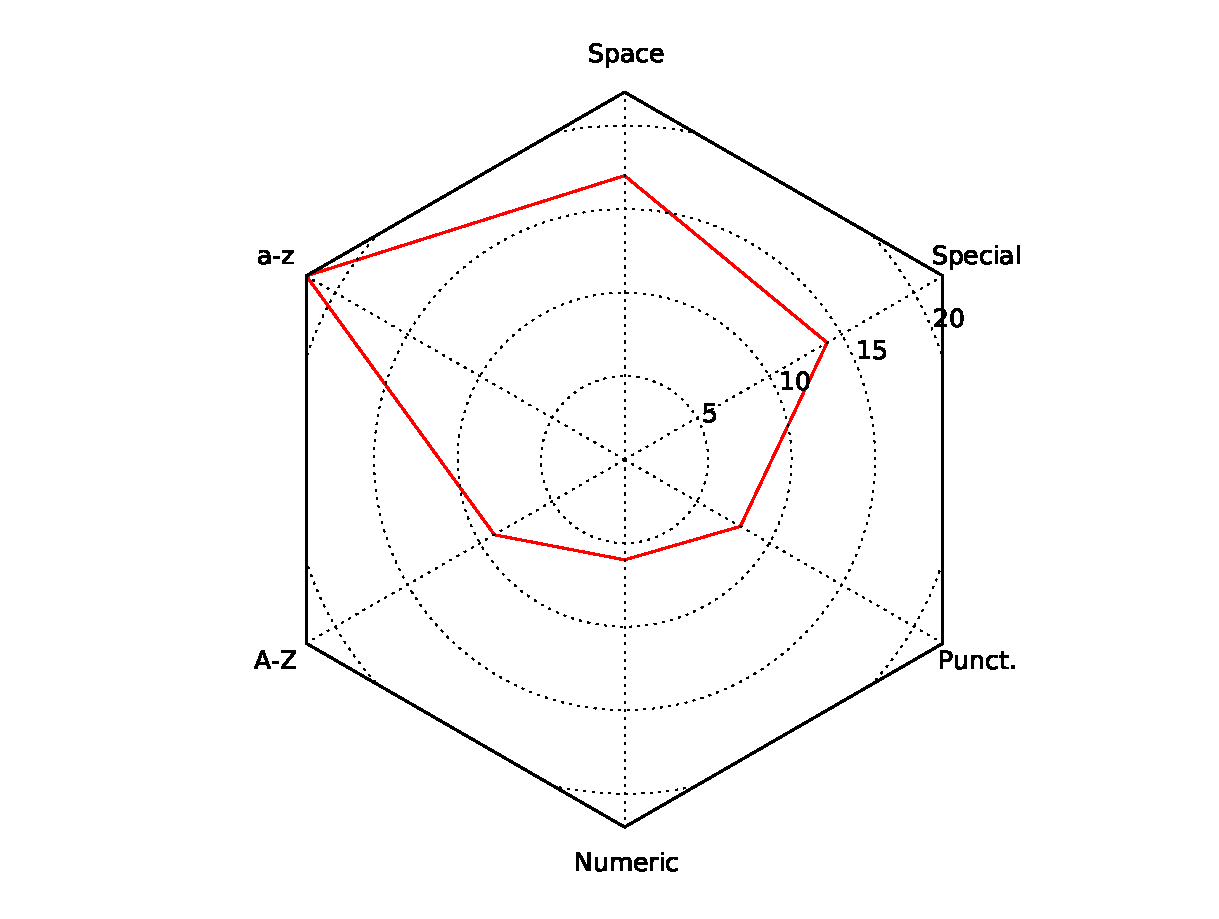
\includegraphics[width=0.5\textwidth]{Figures/body_formula.pdf}} & 
\subfloat[Body (normal)]{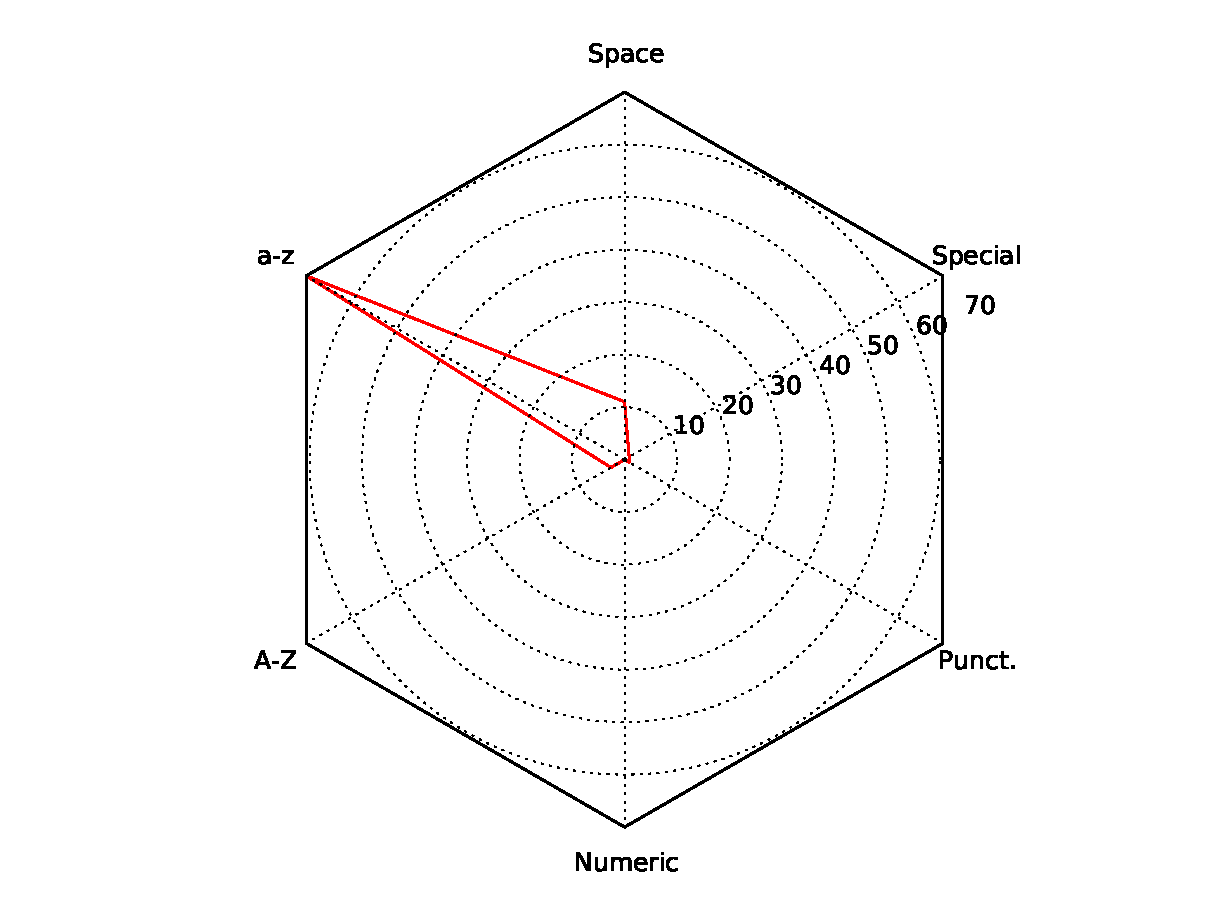
\includegraphics[width=0.5\textwidth]{Figures/body_normal.pdf}}\\
\subfloat[Headnote]{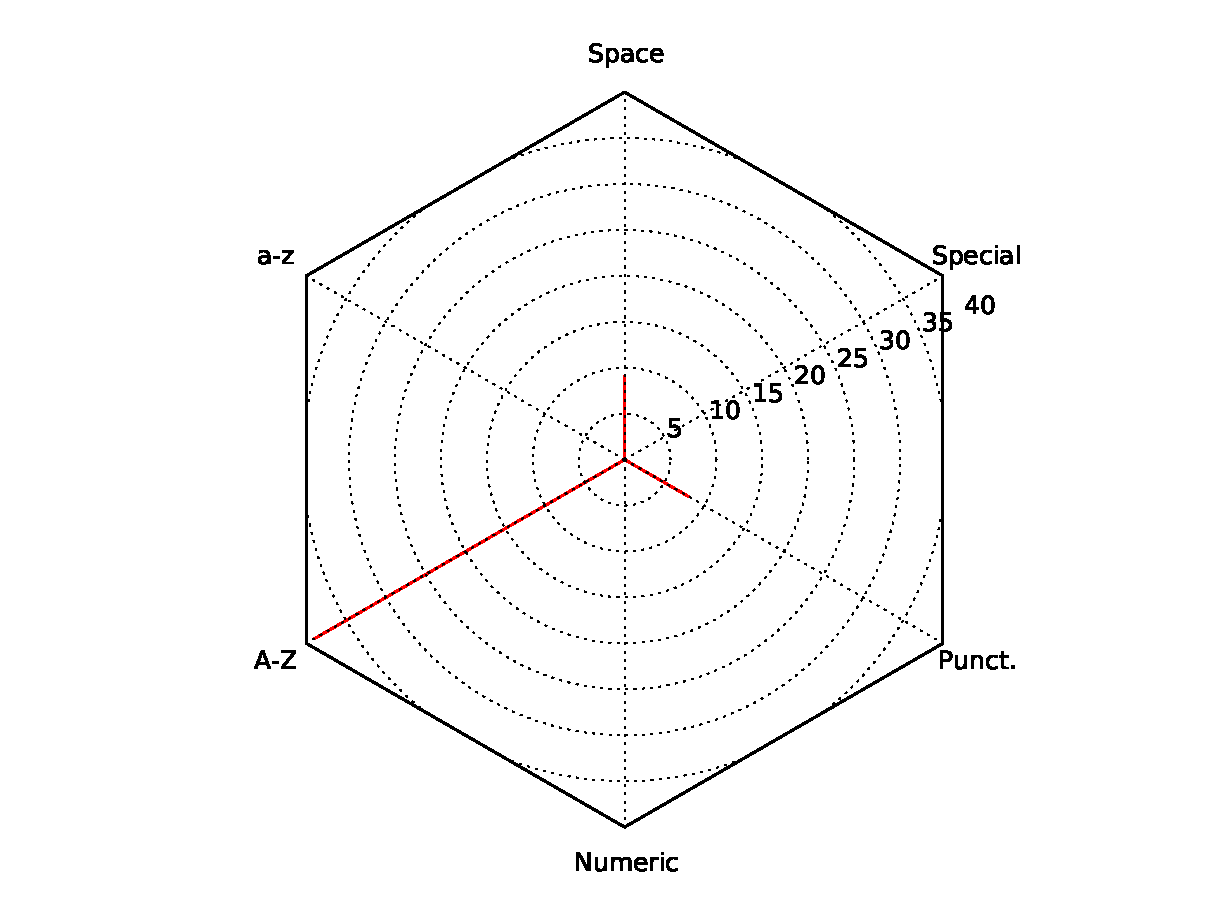
\includegraphics[width=0.5\textwidth]{Figures/headnote.pdf}}&
\subfloat[Page number]{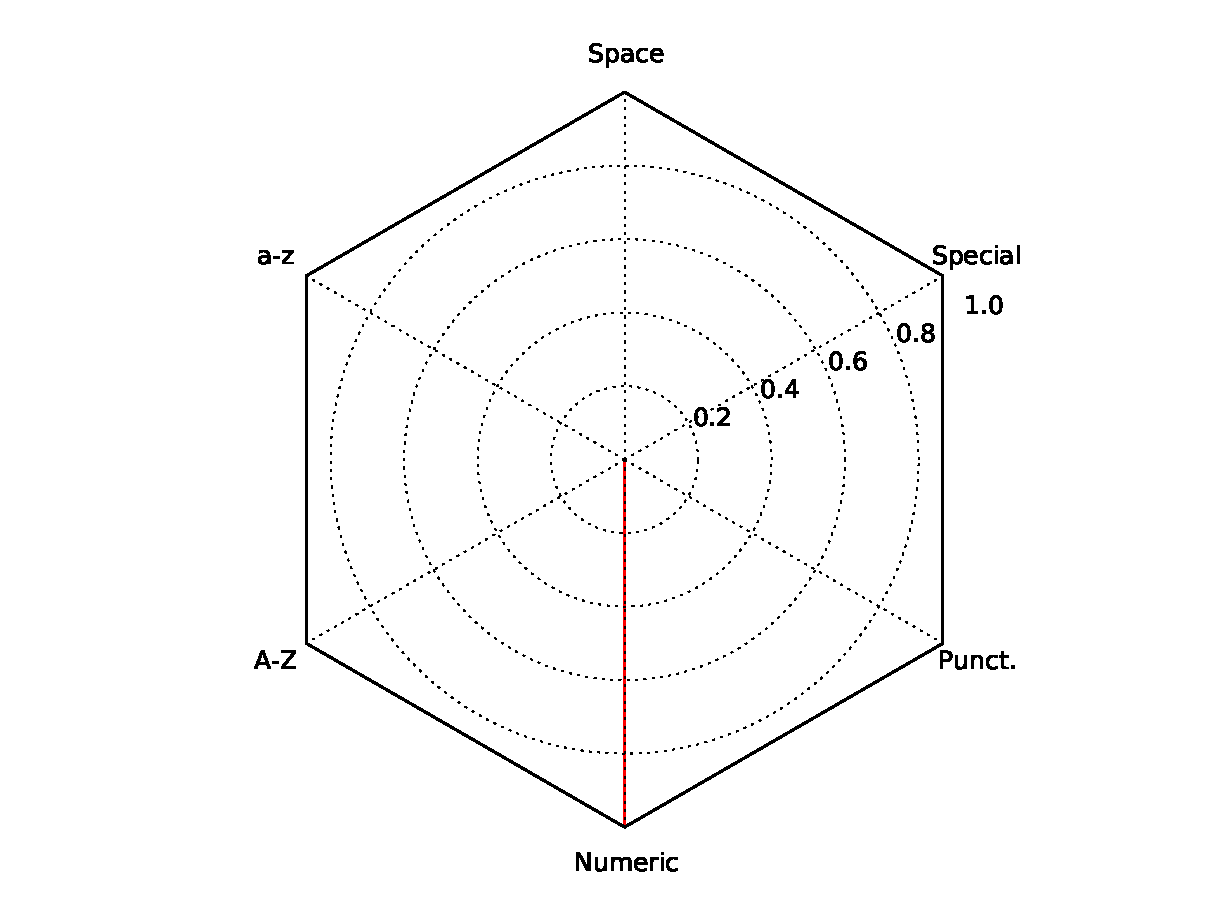
\includegraphics[width=0.5\textwidth]{Figures/page.pdf}} \\
\subfloat[Affilation list]{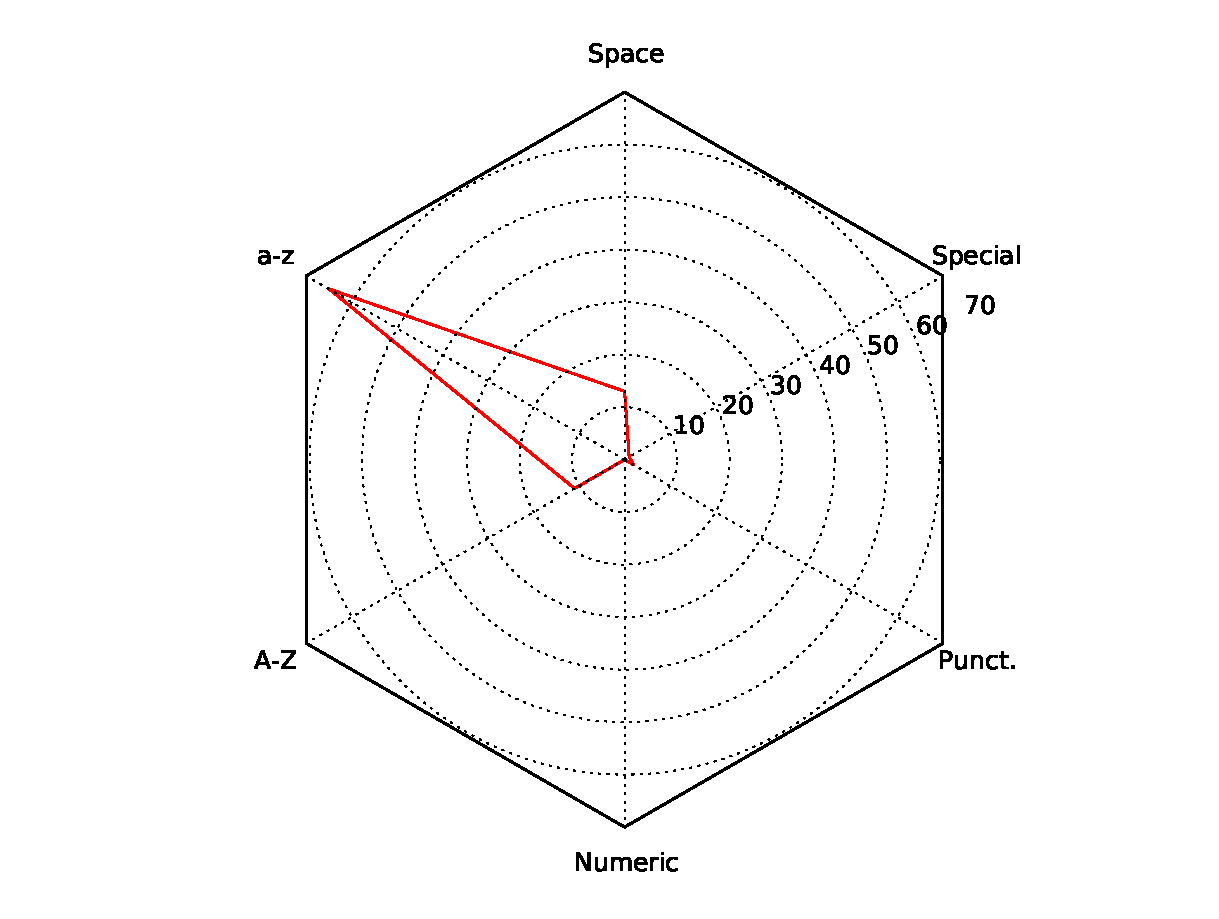
\includegraphics[width=0.5\textwidth]{Figures/affiliations_list.pdf}} & 
\subfloat[Author list]{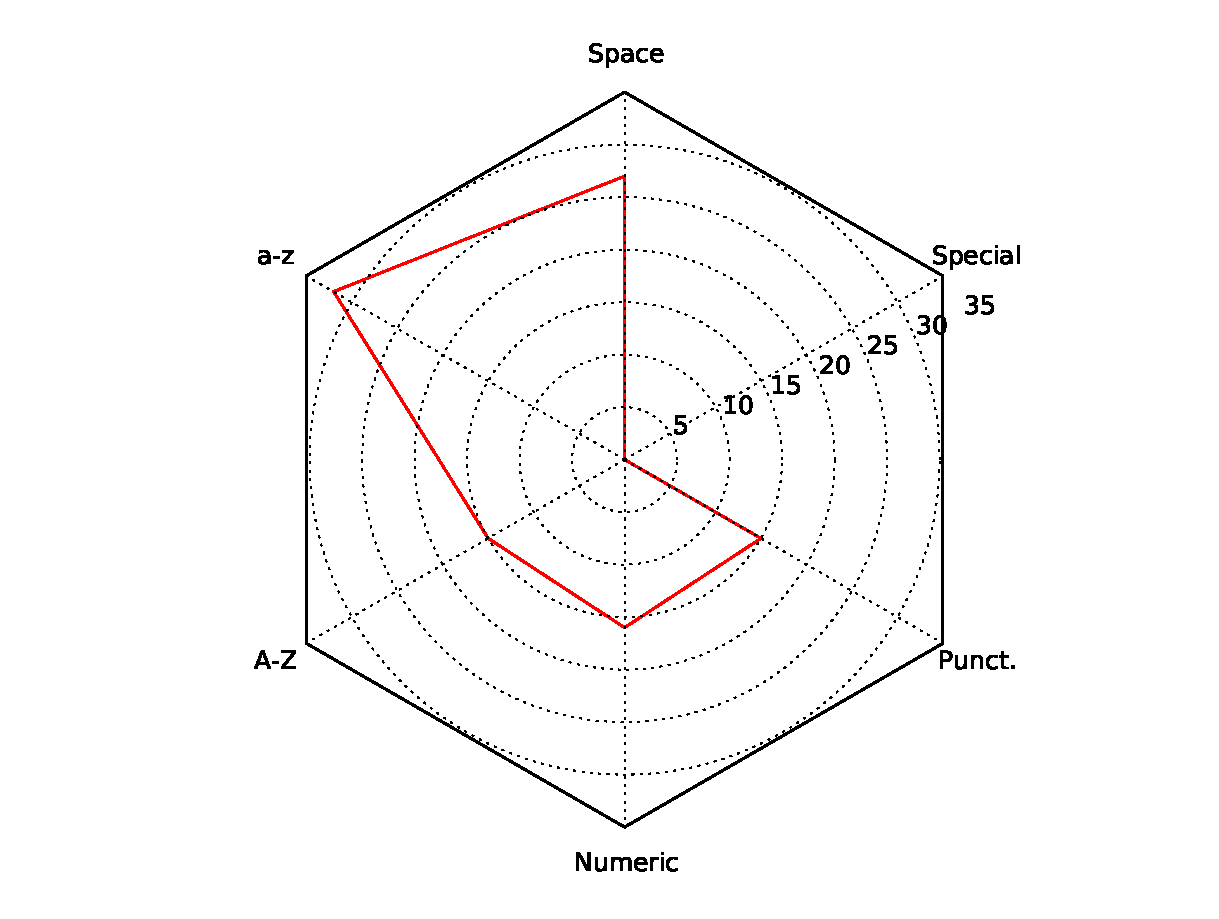
\includegraphics[width=0.5\textwidth]{Figures/author_list.pdf}} \\ 
\end{tabular}
\caption{Character class breakdown of sample lines from different sections of a CERN LHCb collaboration paper. The paper in question is the current world record holder for number of authors, and lists over 5000 authors and their affilations. The radar plots give a different impression for each of the samples.}
\end{figure}
